\chapter{Introduction} 

\label{Introduction}

%----------------------------------------------------------------------------------------
% 											Section 1
\section{Section 1}
Your section content...

You can start your citation here, for example, "in the book \cite{titterton2004strapdown}
\subsection{Sub-section 1}
Your sub-section content...

Example of one figure in one line (Fig. \ref{drone_fig_1})

\begin{figure}
	\centering
	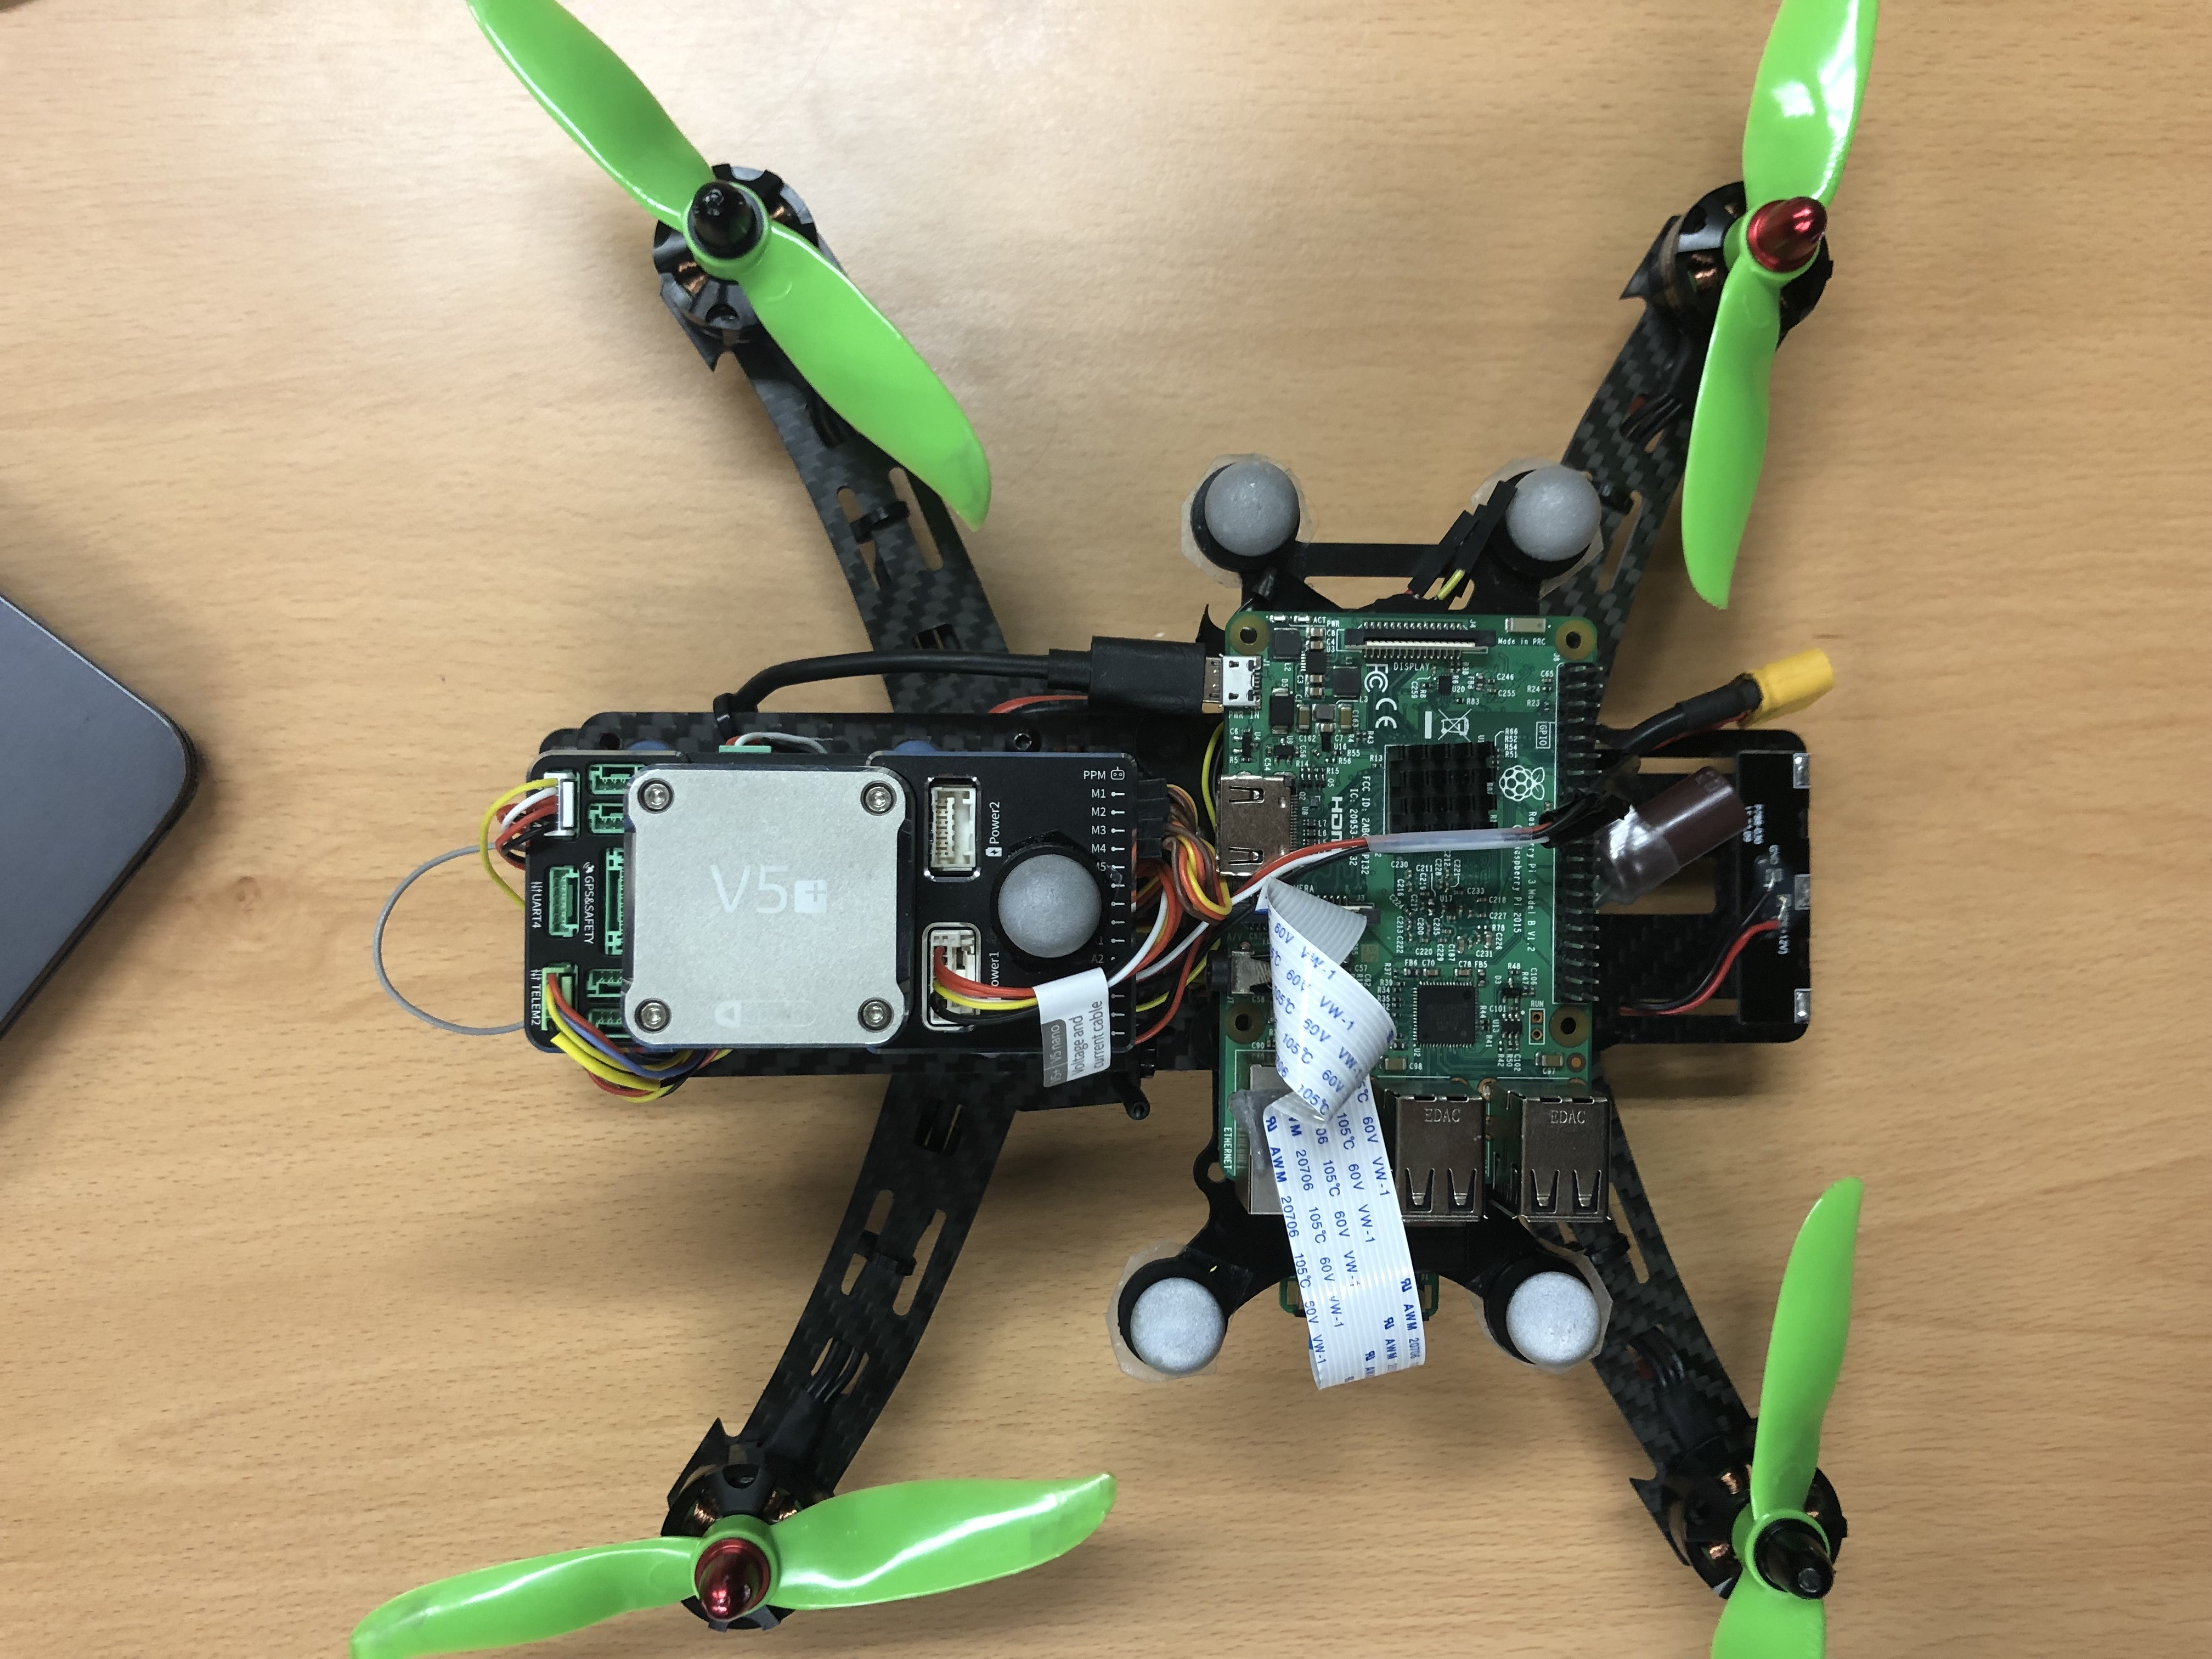
\includegraphics[width=\textwidth,keepaspectratio]{Figures/drone_setup.jpg}
	\caption{caption}
	\label{drone_fig_1}
\end{figure}
	

Example of two figures in one line (Fig. \ref{drone_fig_2})
\begin{figure}
	\centering
	\begin{subfigure}[b]{0.49\textwidth}
		\centering
		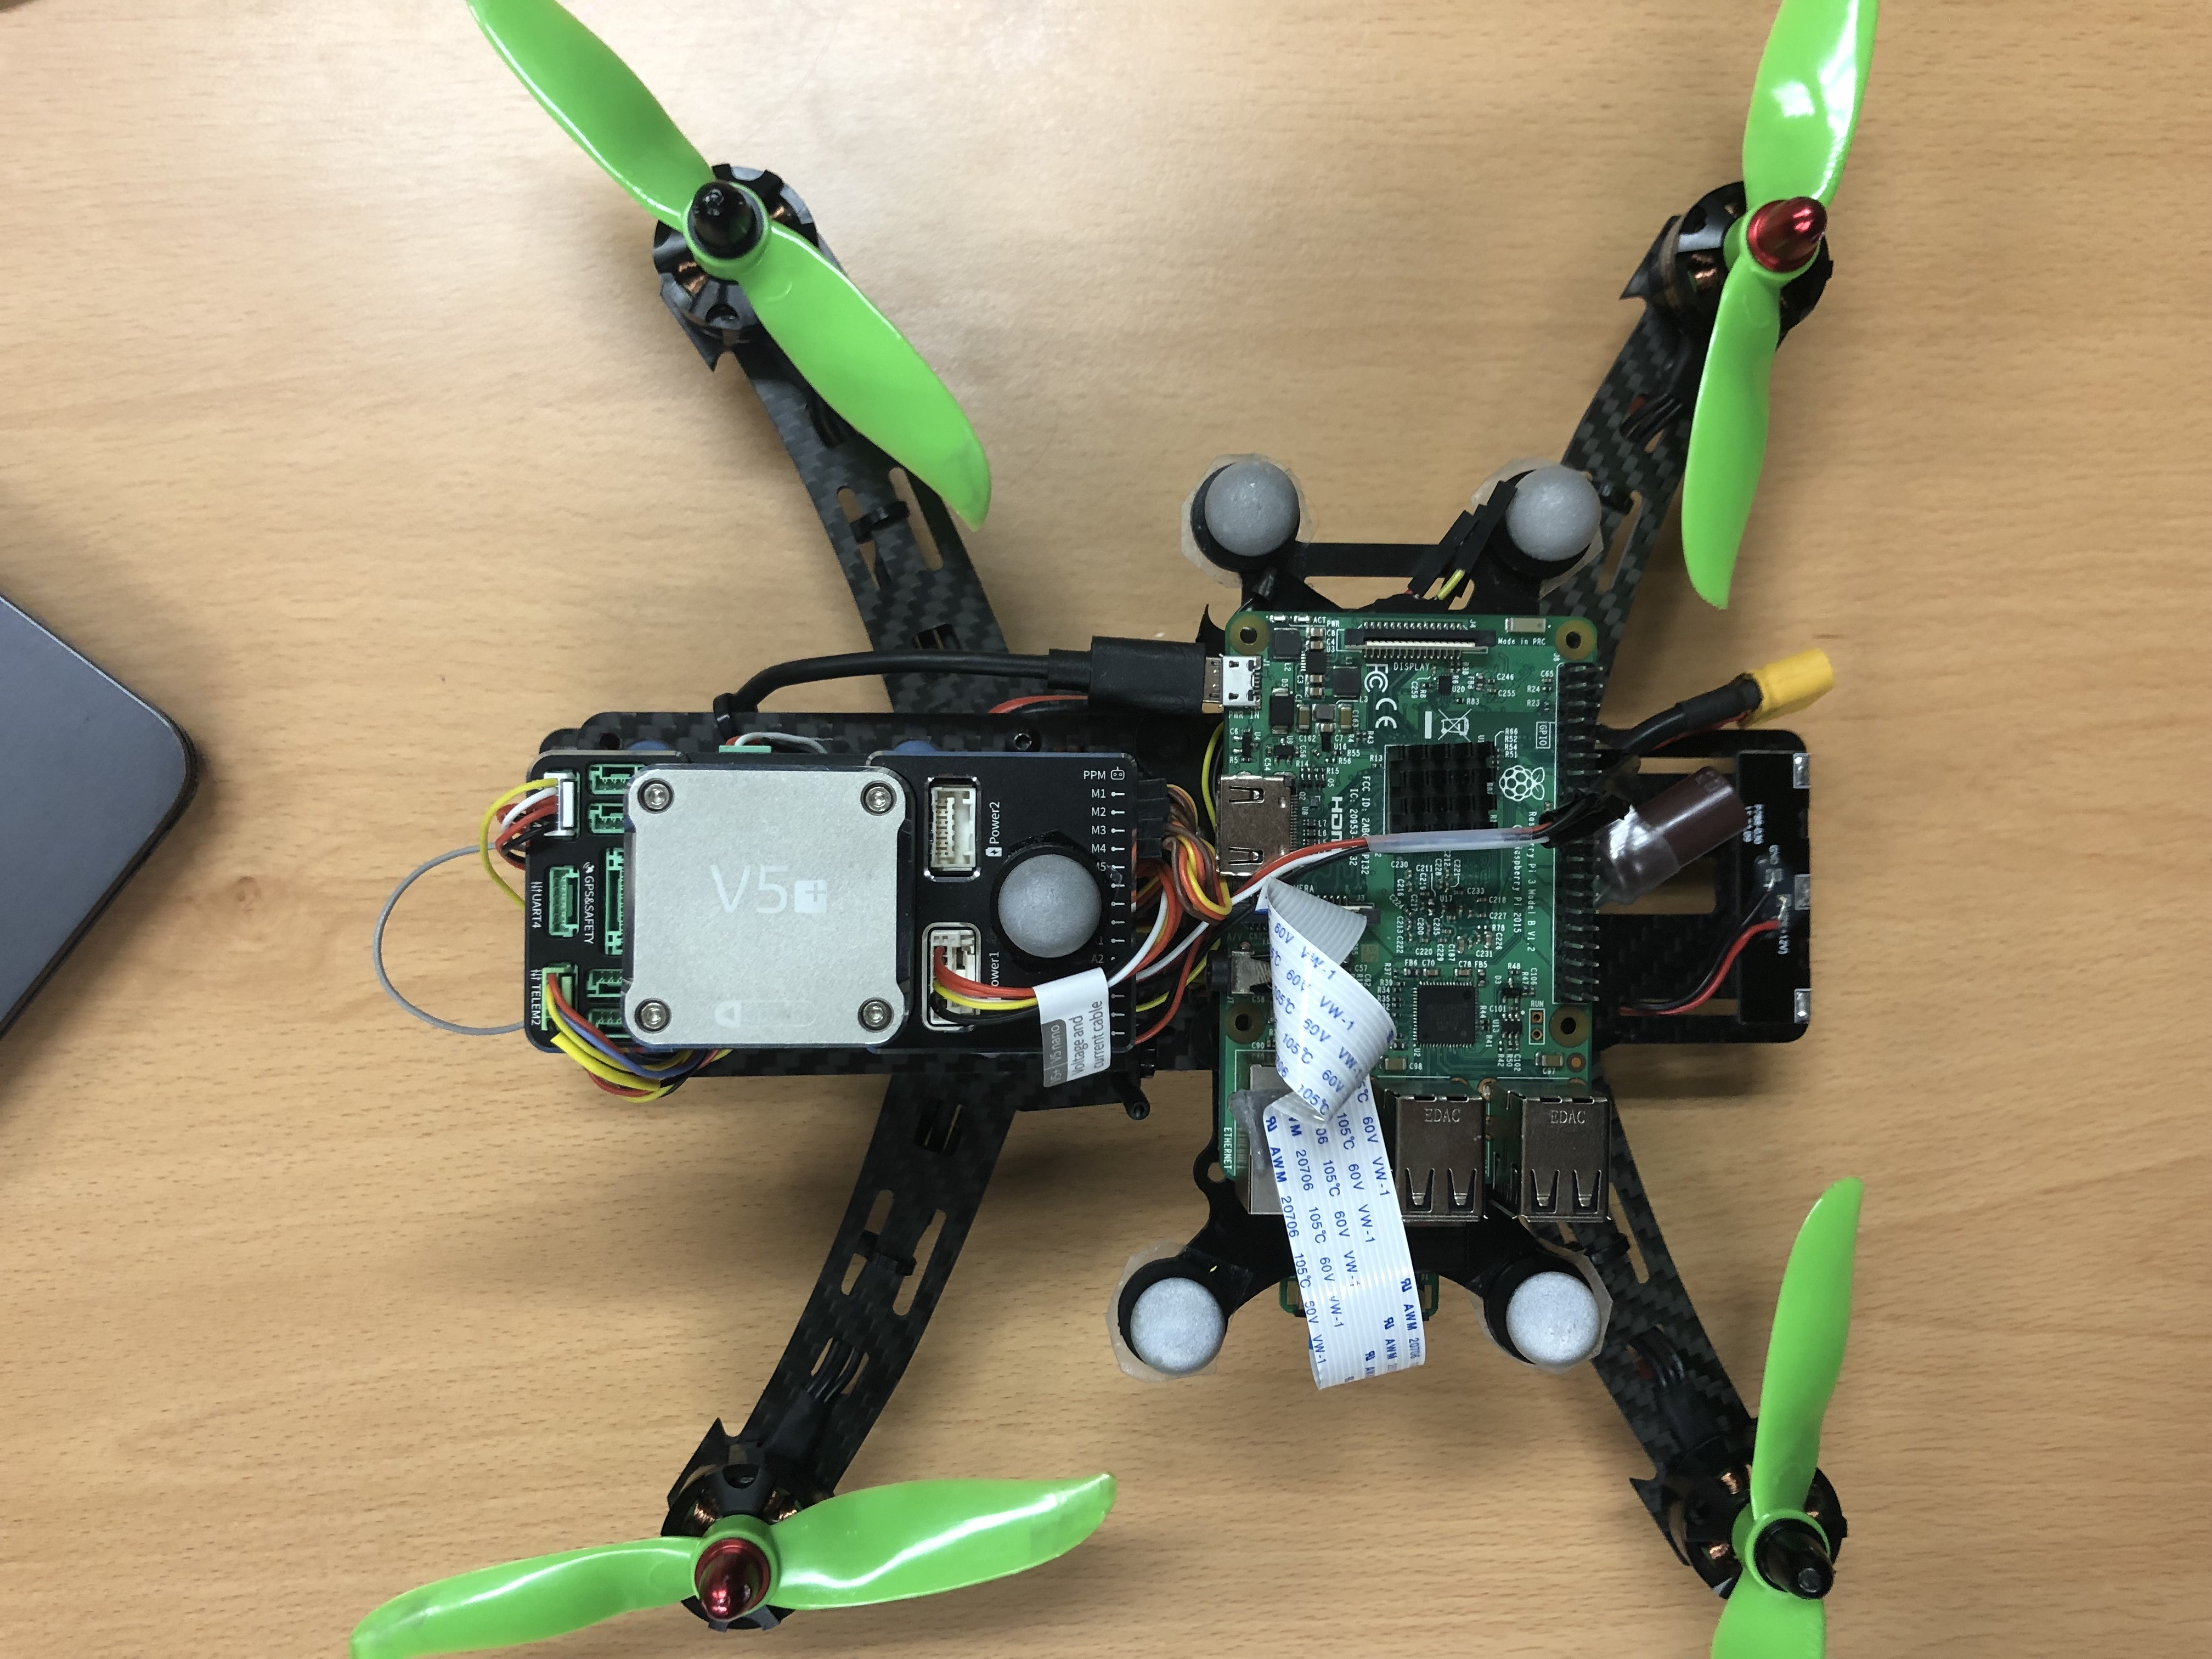
\includegraphics[width=\textwidth,keepaspectratio]{Figures/drone_setup.jpg}
	\end{subfigure}
	\begin{subfigure}[b]{0.49\textwidth}
		\centering
		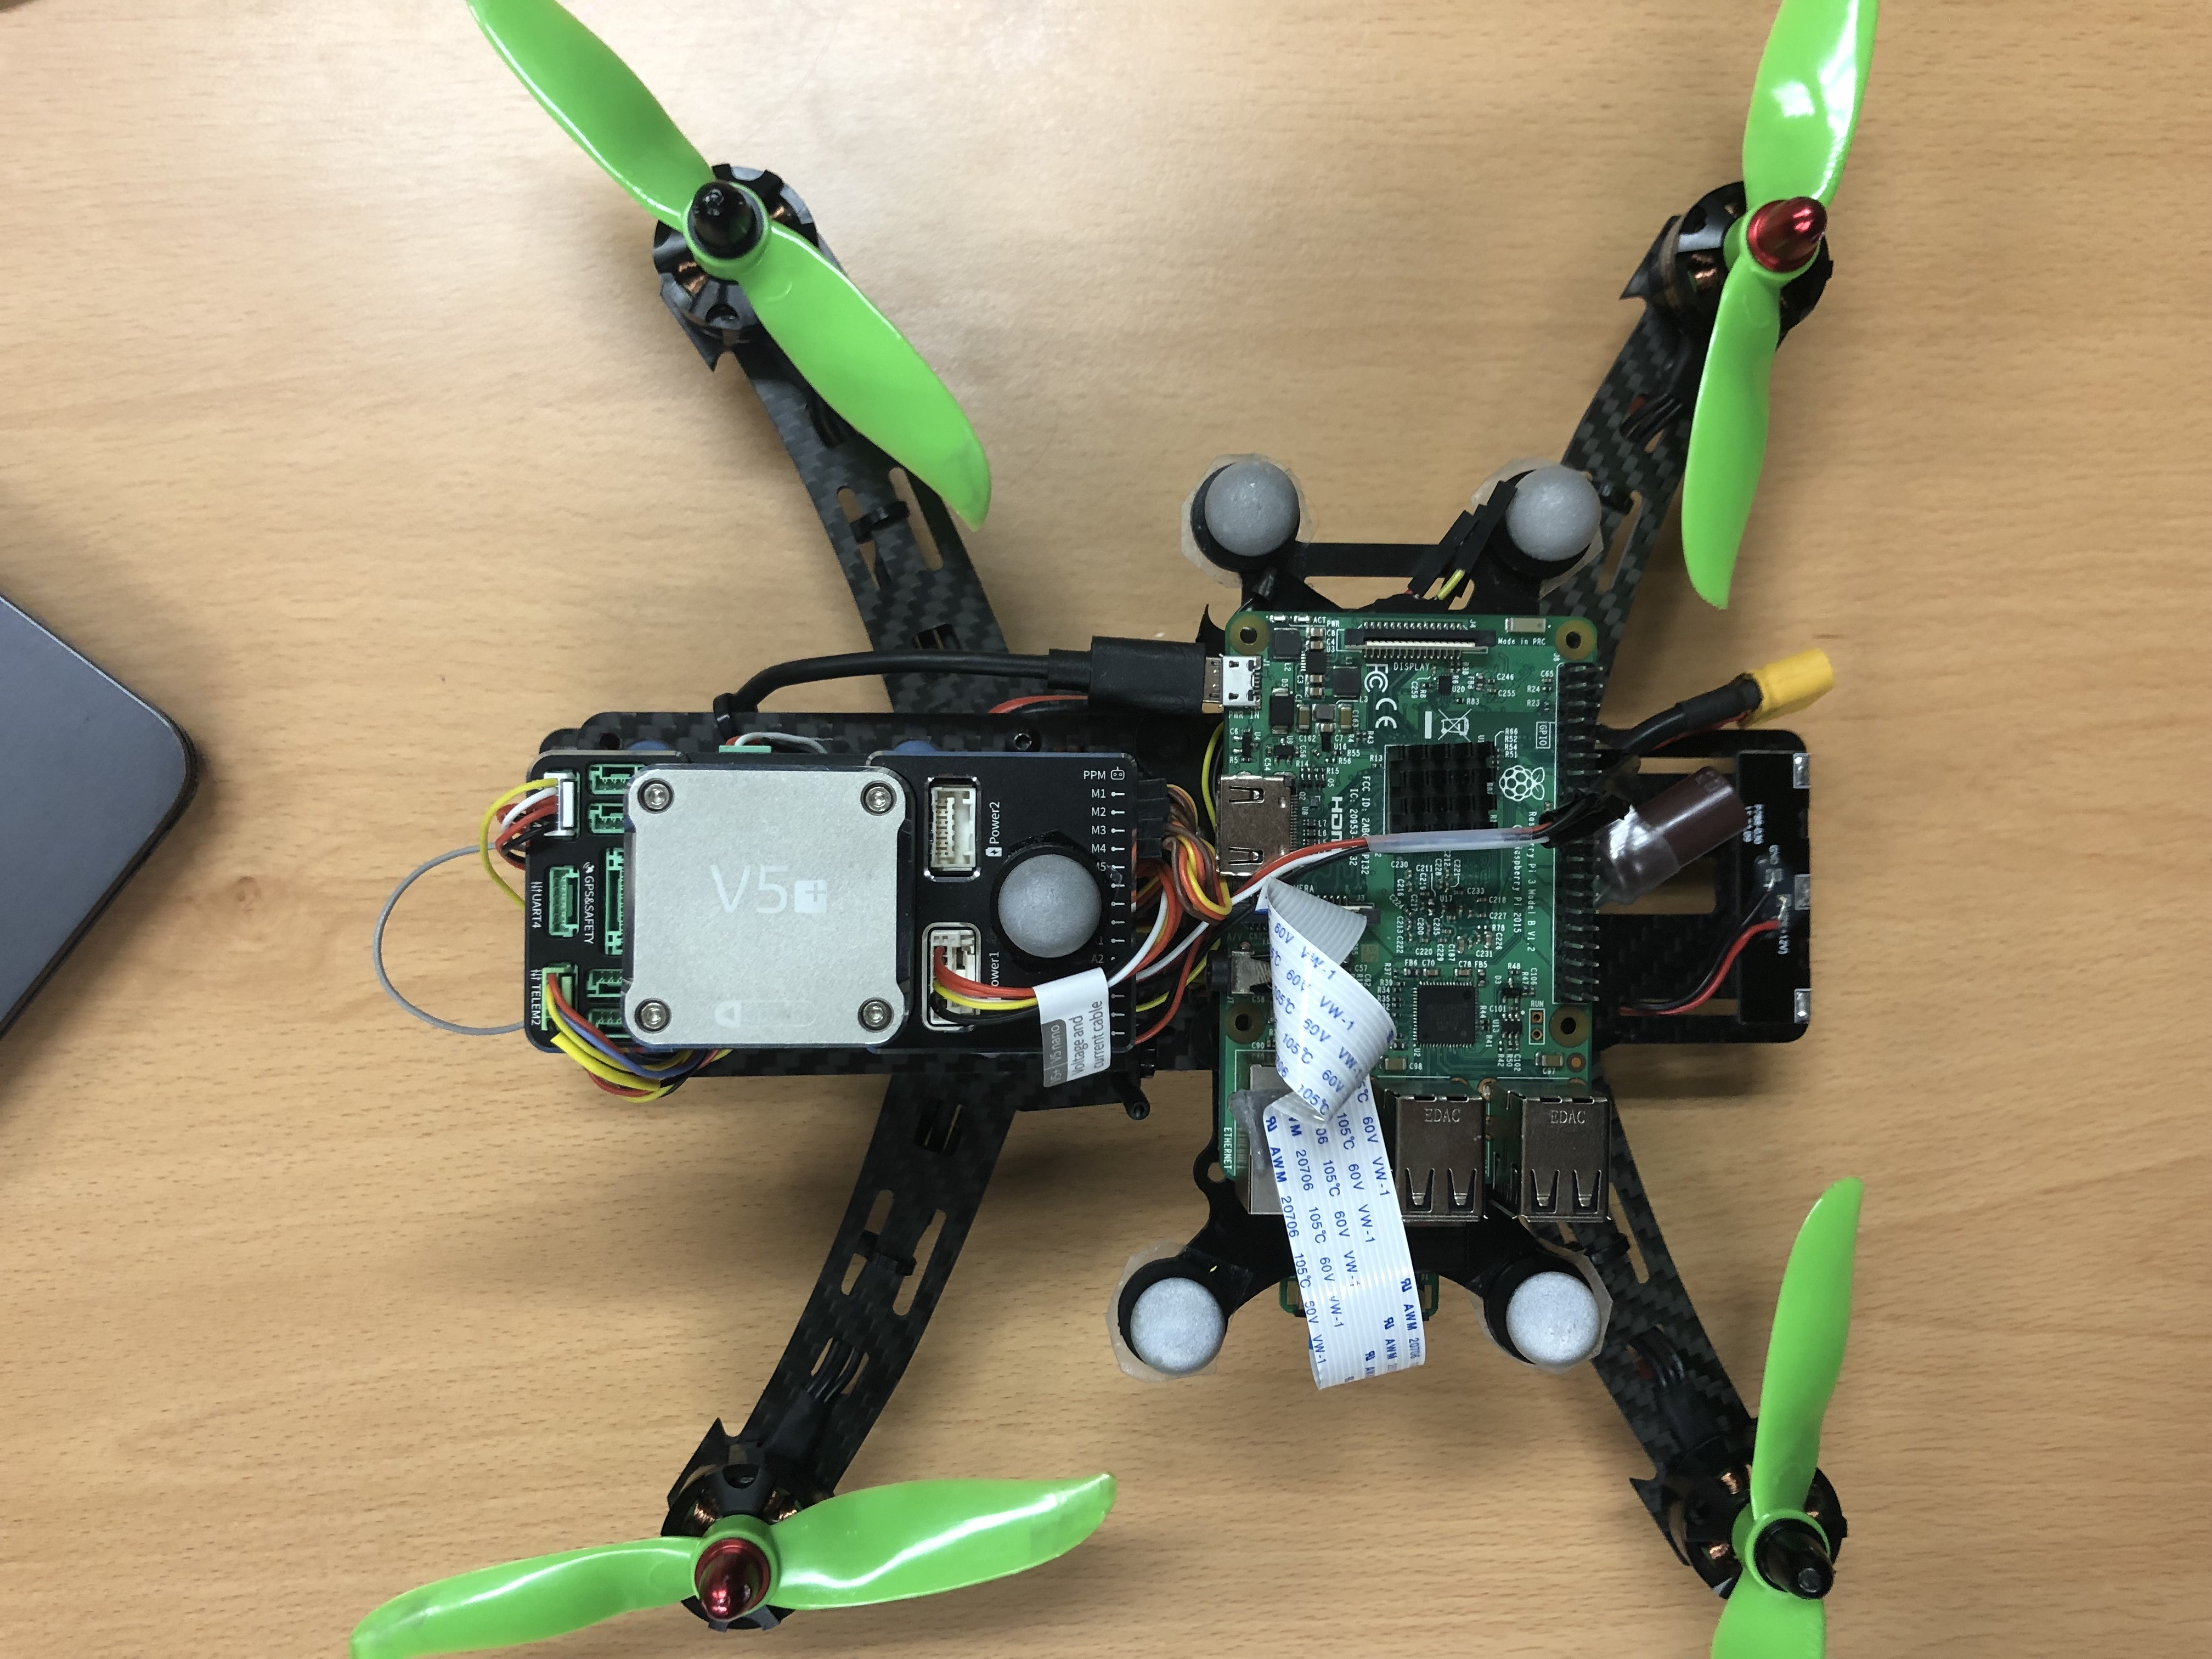
\includegraphics[width=\textwidth,keepaspectratio]{Figures/drone_setup.jpg}
	\end{subfigure}
	\caption{caption}
	\label{drone_fig_2}
\end{figure}

Example of Table \ref{sensors_table} \cite{kys}

\begin{table}[ht]
	\centering
	\setlength{\tabcolsep}{4pt} % Default value: 6pt
	\renewcommand{\arraystretch}{1.5} % Default value: 1
	\begin{tabular}{|c|c|c|}
		\toprule
		& \textbf{Measurement} & \textbf{Drawbacks} \\
		\midrule
		IMU & Linear Accelerations, & Biased and noisy measurements, \\
		& Angular velocities.   & Large uncertain for slow motions.\\
		
		\midrule
		GNSS & Absolute position (outdoor). & Unreliable in indoor \\
		&                              & and urban environments. \\
		\midrule
		Magnetic  & Earth's magnetic  & Disturbed by electronic \\
		Sensor    & field direction.  & devices nearby. \\
		\midrule
		Barometric & Absolute altitude. & Not reliable indoor, \\
		&					& Affected by weather conditions. \\
		\midrule							   
		Camera & Inertial measurement, & Ambiguity, calibration, \\
		& Visual information.   & Affected by light conditions. \\
		
		\midrule
		Laser & Distance to objects & Heavy and expensive, \\
		&  					& 2D information. \\
		\bottomrule
	\end{tabular}
	\caption{Properties of some sensors that are commonly used for estimation task in the literature.}
	\label{sensors_table}
\end{table}

